\chapter{宏观介质静电学}
\label{chap:electrostatics of macroscopic media}

本章内容分为两节:
\begin{compactenum}
    \item \secref{sec:multipole expansion}介绍给定电荷分布系统的电势及其多极展开(multipole expansion),%及处在外场中的电荷系统能量的多极展开。
    多极展开本质是利用逐项逼近的方法来计算电势或能量的,故在系统电荷的空间分布尤为复杂的情况下,使用多极展开去近似计算是一种行之有效的方法。
    
    和某些教材上使用并矢张量的标记法不同,本文使用的是球谐函数表示(通过球谐函数导出也更为自然和简洁)。

    \item \secref{sec:dielectric}介绍了电介质(dielectrics)及含电介质的边值问题。并扼要介绍了分子极化率(atomic polarizability)和宏观电极化率 (susceptibility)的主要特征及彼此之间的关系,导出了 Clausius-Mossotti 方程。最后介绍了含电介质时系统的能量表示。
\end{compactenum}

\section{多极矩展开}
\label{sec:multipole expansion}

电荷的局域(localized)分布由电荷密度$\rho(\bm x')$描述,由式\eqref{eqn:Phi-rho}
\[
    \Phi(\bm x)=\frac1{4\pi\varepsilon_0}\int_V\frac{\rho(\bm x')}{|\bm x'-\bm x|}\d v'.
\]
应用式\eqref{eqn:1/|x-x'|=YY},因为我们对电荷分布之外的电势感兴趣,故$r_<=r',\,r_>=r$
\begin{align}
    \notag
    \Phi(\bm x)&=\frac1{\varepsilon_0}\sum_{\ell=0}^\infty\sum_{m=-\ell}^\ell\frac1{2\ell+1}\biggfkh{\int_V\rho(\bm x'){r'^\ell}Y^\ast_{\ell m}(\theta',\phi')\d v'}\frac{Y_{\ell m}(\theta,\phi)}{r^{\ell+1}}\\
    \label{eqn:Phi multipole}
    &=:\frac1{\varepsilon_0}\sum_{\ell=0}^\infty\sum_{m=-\ell}^\ell\frac{q_{\ell m}}{2\ell+1}\frac{Y_{\ell m}(\theta,\phi)}{r^{\ell+1}}.
\end{align}
其中系数$q_{\ell m}$称为多极矩(multipole moment)
\begin{equation}
    q_{\ell m}:=\int_V\rho(\bm x'){r'^\ell}Y^\ast_{\ell m}(\theta',\phi')\d v'.
\end{equation}
另一方面,也可应用式\eqref{eqn:1/|x-x'|}
\begin{align}
    \notag
    \Phi(\bm x)&=\frac1{4\pi\varepsilon_0}\int_V\rho(\bm x')\sum_{\ell=0}^\infty\frac{r'^\ell}{r^{\ell+1}}P_\ell(\cos\gamma)\d v'\\
    \label{eqn:legendre multipole}
    &=\frac1{4\pi\varepsilon_0}\biggfkh{\frac1r\int_V\rho\d v'+\frac1{r^2}\int_V\rho r'\cos\gamma\d v'+\frac1{r^3}\int_V\rho r'^2P_2(\cos\gamma)\d v'+\cdots},\tag{$\ast$}
\end{align}
前三个积分项分别对应总电荷$q$ (电单极矩,electric monopole moment)、电偶极矩$\bm p$ (dipole)、电四极矩$\mathcal Q_{\alpha\beta}$ (quadrupole):
\begin{align}
    \notag
    q={}&\int_V\rho(\bm x')\d v',\\
    \bm p:={}&\int_V\bm x'\rho(\bm x')\d v',\\
    \mathcal Q_{\alpha\beta}:={}&\int_V(3x_\alpha'x_\beta'-r'^2\vd_{\alpha\beta})\rho(\bm x')\d v'.
\end{align}
则式\eqref{eqn:legendre multipole}可以写成 
\begin{equation}
    \Phi(\bm x)=\frac1{4\pi\varepsilon_0}\biggfkh{\frac qr+\frac{\bm p\cdot\bm r}{r^3}+\frac12\sum_{\alpha,\beta}\frac{\mathcal Q_{\alpha\beta}x_\alpha x_\beta}{r^5}+\cdots}.
\end{equation}
上式也可通过对$1/|\bm x-\bm x'|$在$\bm x'=0$处Taylor展开推导得到。

~

\begin{example}{前几个多极矩}{first few multipole moment}
    易得
    \begin{equation*}
        \begin{aligned}
            q_{00}&=\frac1{\sqrt{4\pi}}\int_V\rho(\bm x')\d v'=\frac1{\sqrt{4\pi}}q;\\
            q_{10}&=-\sqrt{\frac3{8\pi}}\int_V(x'-\i y')\rho(\bm x')\d v'=-\sqrt{\frac3{8\pi}}(p_x-\i p_y),\\
            q_{11}&=-\sqrt{\frac3{4\pi}}\int_V z'\rho(\bm x')\d v'=-\sqrt{\frac3{4\pi}}p_z;
        \end{aligned}
    \end{equation*}
    $q_{1-1}$可由$q_{\ell,-m}=(-)^mq_{\ell m}^\ast$推出,
    \tcblower
    对于任何电荷分布,其最低阶的不为0的多极矩$q_{\ell m}$与原点的选择无关,但剩下所有较高阶的多极矩一般都与原点的位置有关。
\end{example}
\iffalse
由式\eqref{eqn:Phi multipole},电场分量可被表示为
\begin{align*}
    E_r&=-\pv\Phi r=\frac1{\varepsilon_0}\frac{\ell+1}{2\ell+1}q_{\ell m}\frac{Y_{\ell m}(\theta,\phi)}{r^{\ell+2}},\\
    E_\theta&=-\frac1r\pv\Phi\theta=-\frac1{\varepsilon_0}\frac{1}{2\ell+1}q_{\ell m}\frac1{r^{\ell+2}}\pv{Y_{\ell m}(\theta,\phi)}\theta,\\
    E_\phi&=-\frac1{r\sin\theta}\pv\Phi\phi=-\i\frac1{\varepsilon_0}\frac{1}{2\ell+1}q_{\ell m}\frac1{r^{\ell+2}}\frac{m}{\sin\theta}{Y_{\ell m}(\theta,\phi)},
\end{align*}
\fi
\begin{example}{等量异号电荷对的电场}{E of pm q}
    考虑位于$z$轴坐标分别为$\pm a$的等量异号电荷对$\pm q$,其在空间激发的电势为
    \begin{align*}
        \Phi&=\frac q{4\pi\varepsilon_0}\biggfkh{\frac1{\sqrt{a^2+r^2-2ar\cos\theta}}-\frac1{\sqrt{a^2+r^2+2ar\cos\theta}}}\\
        &=\frac q{4\pi\varepsilon_0r}\sum_{\ell=0}^\infty\Bigkh{\frac ar}^\ell\bigfkh{P_{\ell}(\cos\theta)-P_\ell(-\cos\theta)}\\
        &=\frac q{4\pi\varepsilon_0r}\biggfkh{\frac{2a}r\cos\theta+\Bigkh{\frac ar}^3(5\cos^3\theta-3\cos\theta)+\cdots}
    \end{align*}
    对于$r\gg a$的远场,仅保留第一项,与理想电偶极矩$p:=q\cdot 2a$相同
    \begin{equation}
        \label{eqn:edipole-Phi}
        \Phi(r,\theta)=\frac{p\cos\theta}{4\pi\varepsilon_0r^2},
    \end{equation}
    相应的电场为
    \begin{align}
        \label{eqn:edipole-E}
        \bm E(r,\theta)&=\frac{p}{4\pi\varepsilon_0r^3}(2\cos\theta\uvec r+\sin\theta\uvec\theta).
    \end{align}
\end{example}
若电偶极子处于$\bm x_0$,电场为 
\begin{equation}
    \label{eqn:edipole-E without delta}
    \bm E(\bm x)=-\nabla\Phi=\frac{3(\bm p\cdot\uvec n)\uvec n-\bm p}{4\pi\varepsilon_0|\bm x-\bm x_0|^3},\quad \uvec n:=\frac{\bm x-\bm x_0}{|\bm x-\bm x_0|}.
    \tag{$\star$}
\end{equation}
式\eqref{eqn:edipole-E without delta}并不严格,事实上在含$\bm x_0$处积分会产生额外的项,应进行修正:
\begin{equation}
    \label{eqn:edipole-E with delta}
    \bm E(\bm x)=\frac1{4\pi\varepsilon_0}\biggfkh{\frac{3(\bm p\cdot\uvec n)\uvec n-\bm p}{|\bm x-\bm x_0|^3}-\frac{4\pi}3\bm p\vd(\bm x-\bm x_0)}.
\end{equation}

\subsection{能量的多极矩展开}
\label{ssec:multipole expansion of energy}

系统的静电能为
\[
    W=\int_V\rho(\bm x)\Phi(\bm x)\d v
\]
对$\Phi(\bm x)$在原点处Taylor展开
\[
    \Phi(\bm x)=\Phi(\bm 0)-\bm x\cdot\bm E(\bm 0)-\frac12\sum_{\alpha,\beta}x_\alpha x_\beta\pv{E_\beta}{x_\alpha}(\bm 0)+\cdots
\]
得到 
\begin{equation}
    W=q\Phi(\bm 0)-\bm p\cdot\bm E(\bm 0)-\frac16\sum_{\alpha,\beta}\mathcal Q_{\alpha\beta}\pv{E_\beta}{x_\alpha}(\bm 0)+\cdots
\end{equation}
多极子和外场相互作用的特征方式:电荷与电位、电偶极子与电场、电四极子与电场梯度……

两个电偶极子之间的互能
\begin{equation}
    W_{12}=\frac{\bm p_1\cdot\bm p_2-3(\uvec n\cdot\bm p_1)(\uvec n\cdot\bm p_2)}{4\pi\varepsilon_0|\bm x_1-\bm x_2|^3},\quad\uvec n:=\frac{\bm x_1-\bm x_2}{|\bm x_1-\bm x_2|}.
\end{equation}
\paragraph{电偶极子的能量、力矩和力}对$\bm E$展开至一阶项,得到电偶极子在电场中受到的力为
\begin{equation}
    \bm F=\int_V\rho\bm E\d v\simeq(\bm p\cdot\nabla)\bm E,
\end{equation}
一般地,$\bm p$不随坐标变化,上式也可写成$\nabla(\bm p\cdot\bm E)$: 
\begin{align*}
    \nabla(\bm p\cdot\bm E)&=\bm p\times\cancel{(\curl\bm E)}+\bm E\times\cancel{(\curl\bm p)}+(\bm p\cdot\nabla)\bm E+\cancel{(\bm E\cdot\nabla)\bm p}.
\end{align*}
利用\exmref{exm:E of pm q} 中的模型,可以很直观地推出电偶极子在电场中受到的力矩为
\begin{equation}
    \bm N=\bm p\times\bm E,
\end{equation}
由$\bm F=-\nabla U$,可定义电偶极子在电场中的势能为
\begin{equation}
    U=-\bm p\cdot\bm E.
\end{equation}

\section{电介质}
\label{sec:dielectric}

电介质(dielectric)是能够被电极化的绝缘体。与导体的自由电荷不同,电介质的带电粒子被原子、分子的内力或分子间的力紧密束缚着,称为束缚电荷(bound charge)。在外电场作用下,这些电荷也只能在微观范围内移动,产生极化(polarization)。
极化主要有三种机制:
\begin{compactenum}
    \item 畸变极化:原子核外的电子云分布产生畸变,从而产生不等于零的电偶极矩;
    \item 位移极化:分子原来正负电中心重合,在外电场作用下正负电中心分离产生电偶极矩;
    \item 转向极化:分子有固有电偶极矩,但取向混乱,宏观上电偶极矩总和等于零。在外电场作用下,各个电偶极子趋向于一致的排列,从而宏观电偶极矩不等于零。
\end{compactenum}
在静电场中,电介质内部可以存在电场,这是电介质与导体的基本区别。
\paragraph{宏观电场}
在前一章中,我们没有考虑有质介质(ponderable media)的存在,所以我们没有区分微观场(microscopic)和宏观场(macroscopic)。
但是静电学主要涉及有质介质中的电荷和场,因此%它们各自的电响应必须考虑在内:(1)分子电荷密度会被扭曲。(2)每个分子的多极矩都是不同的。
我们必须在微观层面上考虑有质介质的极化效应(polarization effect)。为了得到适用于宏观现象的Maxwell方程,我们对宏观小、微观大的区域求平均:% 在第6章中,我们只会小心翼翼地做到这一点
\begin{equation}
    \label{eqn:curlE-macro}
    \curl\bm E_\text{micro}=\bm 0\implies\curl\bm E=\bm 0.
\end{equation}
方程对求平均后的宏观电场$\bm E$适用。这意味着电场仍然可以从静电学中的电势推导出来。

%如果电场作用于由大量原子(或分子)组成的介质,束缚在每个分子中的电荷将执行摄动运动(perturbed motions),由此在介质中产生了电极化。
在多极子与电场的作用中,偶极子占主导地位。定义电极化强度(electric polarization) $\bm P$为单位体积的偶极矩
\begin{equation}
    \bm P:=\sum_i N_i\ave{\bm p_i}.
\end{equation}
假设更高阶的宏观多极矩密度可忽略,则有质介质的电势为
\begin{align*}
    \D\Phi(\bm x,\bm x')&=\frac1{4\pi\varepsilon_0}\biggfkh{\frac{\rho(\bm x')}{|\bm x-\bm x'|}\D V+\frac{\bm P(\bm x')\cdot(\bm x-\bm x')}{|\bm x-\bm x'|^3}\D V}\\
    &=\frac1{4\pi\varepsilon_0}\biggfkh{\frac{\rho(\bm x')}{|\bm x-\bm x'|}+\bm P(\bm x')\cdot\nabla'\biggkh{\frac1{|\bm x-\bm x'|}}}\D V
\end{align*}
变成积分并应用分部积分得到
\begin{equation}
    \Phi(\bm x)=\frac1{4\pi\varepsilon_0}\int_V\frac{\rho(\bm x')-\div\bm P(\bm x')}{|\bm x-\bm x'|}\d v'.
\end{equation}
$\rho$是自由电荷(或过剩电荷)密度,
$\rho_\text{pol}:=-\div\bm P$是极化电荷密度。%上式是由电荷分布$(\rho-\div\bm P)$激发电势的习惯表达式。
从而
%由$\bm E=-\nabla\Phi$,第一个Maxwell方程为 
\begin{equation}
    \label{eqn:divE-P}
    \div\bm E=-\lapla\Phi=\frac{\rho-\div\bm P}{\varepsilon_0}.
\end{equation}
若极化不均匀,任何小体积内的电荷都会有净增加或净减少,这就是为什么存在$\div\bm P$的原因。

将式\eqref{eqn:divE-P}移项,可定义电位移矢量(electric displacement)
\begin{equation}
    \bm D:=\varepsilon_0\bm E+\bm P.
\end{equation}
从而式\eqref{eqn:divE-P}变为 
\begin{equation}
    \label{eqn:divD}
    \div\bm D=\rho.
\end{equation}
式\eqref{eqn:curlE-macro}和\eqref{eqn:divD}是式\eqref{eqn:curlE}和\eqref{eqn:divE}的宏观对应。
\paragraph{本构关系}
为了解Maxwell方程组,我们需要找到$\bm D$和$\bm E$之间的本构关系(constitutive relation)。为了简化,我们假设介质是各向同性的(isotropic),且系统对外加场的响应是线性的(linear)。因此
\begin{equation}
    \bm P=\varepsilon_0\chi_\elc\bm E.
\end{equation}
其中$\chi_\elc$称为介质的电极化率(electric susceptibility)。由此得到 
\begin{equation}
    \bm D=\varepsilon\bm E,\quad \varepsilon:=\varepsilon_0(1+\chi_\elc)=:\varepsilon_\r\varepsilon_0.
\end{equation}
$\varepsilon_\r:=1+\chi_\elc$称为介电常数(dielectric constant)或相对介电常数(relative electric permittivity)。

如果电介质不仅是各向同性的,而且是均匀的,则$\varepsilon$与位置无关。式\eqref{eqn:divE-P}可被写为 
\begin{equation}
    \div\bm E=\frac\rho\varepsilon.
\end{equation}
%各向同性
均匀电介质中的所有问题都可归结为前几章的问题,仅需做替换:
\begin{equation}
    \bm E'=\frac{\varepsilon_0}\varepsilon\bm E,\quad C'=\frac\varepsilon{\varepsilon_0}C.
\end{equation}
\paragraph{表面分布}
考虑介质界面上$\bm D$和$\bm E$的分布,我们可以得到:
\begin{align}
    \label{eqn:Dn2-Dn1}
    (\bm D_2-\bm D_1)\cdot\uvec n_{21}&=\sigma,\\
    \label{eqn:Et2-Et1}
    (\bm E_2-\bm E_1)\times\uvec n_{21}&=\bm 0,
\end{align}
$\uvec n_{21}$是边界上从区域(1)指向区域(2)的法向量;$\sigma$是宏观表面电荷密度(不包含极化电荷)。

边界上表面极化电荷密度$\sigma_\text{pol}$的关系为
\begin{equation}
    \label{eqn:Pn2-Pn1}
    -(\bm P_2-\bm P_1)\cdot\uvec n_{21}=\sigma_\text{pol}.
\end{equation}
对于非均匀介质,极化电荷在介质内部随处可见;对于均匀介质,极化电荷仅位于自由电荷附近和两种不同介质之间的界面处;极化电荷所在的界面不是理想的几何界面,实际上,它们的厚度包含了几层分子。

\subsection{含电介质的边值问题}
\label{ssec:boundary-value problem with dielectrics}

我们可以推广之前介绍的方法来解决电介质的问题。
\begin{example}{电介质中的镜像电荷}{method of images, dielectrics}
    半无限电介质$\varepsilon_1$与半无限电介质$\varepsilon_2$被隔开,
    考虑嵌入在$\varepsilon_1$中的点电荷$q$距离边界$d$,如图所示。
    \begin{center}
        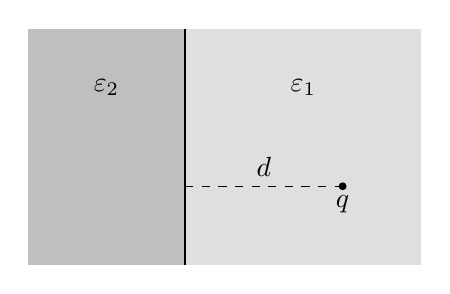
\begin{tikzpicture}
            \fill[gray!25](0, 0)rectangle(3, 3);
            \fill[gray!50](0, 0)rectangle(-2, 3);
            \node at(1.5, 2.25){$\varepsilon_1$};
            \node at(-1, 2.25){$\varepsilon_2$};
            \draw[thick](0, 0)--(0, 3);
            \draw[dashed](0, 1)--(2, 1)node[midway, above]{$d$};
            \fill[black](2, 1)circle(.05)node[below]{$q$};
        \end{tikzpicture}
        \captionof{figure}{电介质中的电荷}
    \end{center}
    为了计算$z>0$部分的电位,在$z<0$部分与$q$对称的位置放置镜像电荷$q'$:
    \[
        \Phi_1=\frac1{4\pi\varepsilon_1}\biggkh{\frac q{R_1}+\frac{q'}{R_2}},\quad z>0;
    \]
    为了计算$z<0$部分的电位,在$q$的位置替换为镜像电荷$q''$:
    \[
        \Phi_2=\frac1{4\pi\varepsilon_2}\frac{q''}{R_1},\quad z<0.
    \]
    由边界条件: 
    \begin{align*}
        \begin{cases}
            \varepsilon_1E_{1z}=\varepsilon_2E_{2z}\\
            E_{1\rho}=E_{2\rho}
        \end{cases}\implies
        \begin{cases}
            q-q'=q''\\
            \frac{q+q'}{\varepsilon_1}=\frac{q''}{\varepsilon_2}
        \end{cases}\implies
        \begin{cases}
            q'=-\frac{\varepsilon_2-\varepsilon_1}{\varepsilon_2+\varepsilon_1}q\\[1ex]
            q''=\frac{2\varepsilon_2}{\varepsilon_2+\varepsilon_1}q
        \end{cases}
    \end{align*}
    $\varepsilon_2>\varepsilon_1$时,$q,q'$符号相反,$\varepsilon_1$内的电场线外凸;
    
    $\varepsilon_2<\varepsilon_1$时,$q,q'$同号,$\varepsilon_1$内电场线内凸。
    \tcblower 
    由式\eqref{eqn:Pn2-Pn1},$z=0$上极化电荷面密度为
    %\bm P_i=(\varepsilon_i-\varepsilon_0)\bm E_i=-(\varepsilon_i-\varepsilon_0)\nabla\Phi(0^\pm).
    \[
        \sigma_\text{pol}=P_{2z}-P_{1z}=-\frac q{2\pi}\frac{\varepsilon_0(\varepsilon_2-\varepsilon_1)}{\varepsilon_1(\varepsilon_2+\varepsilon_1)}\frac d{(\rho^2+d^2)^{3/2}}.
    \]
    当$\varepsilon_2\gg\varepsilon_1$时,介质$\varepsilon_2$表现很像导体($q'=-q$)。
\end{example}
\begin{example}{匀强电场中的介质球}{dielectric sphere in uniform electric field}
    半径为$a$的介质球$\varepsilon$在匀强电场$E_0$中。其电势
    \begin{alignat*}{2}
        \Phi_1&=\sum_{\ell=0}^\infty A_\ell r^\ell P_\ell(\cos\theta),&\quad&r<a\\
        \Phi_2&=\sum_{\ell=0}^\infty\bigfkh{B_\ell r^\ell+C_\ell r^{-(\ell+1)}}P_\ell(\cos\theta),&&r>a
    \end{alignat*}
    又$r\to\infty$时,$\Phi_2\simeq -E_0r\cos\theta$,故 
    \[
        \Phi_2=-E_0r\cos\theta+\sum_{\ell=0}^\infty C_\ell r^{-(\ell+1)}P_\ell(\cos\theta),
    \]
    由边界条件……
    \[
        \Phi=\begin{cases}
            -\frac{3}{\varepsilon_\r+2}E_0r\cos\theta,&r<a\\
            -E_0r\cos\theta+\biggkh{\frac{\varepsilon_\r-1}{\varepsilon_\r+2}}E_0\frac{a^3}{r^2}\cos\theta,&r>a
        \end{cases}
    \]
    因此介质球内是匀强电场
    \[
        E_\text{in}=\frac{3}{\varepsilon_\r+2}E_0;
    \]
    介质球外相当于外加场$E_0$加上原点的电偶极场,偶极矩朝向电偶极场的方向
    \[
        \bm p=4\pi\varepsilon_0\biggkh{\frac{\varepsilon_\r-1}{\varepsilon_\r+2}}a^3\bm E_0,
    \]
    球体内的电极化强度
    \begin{equation}
        \label{eqn:P-E}
        \bm P=(\varepsilon-\varepsilon_0)\bm E_\text{in}=3\varepsilon_0\biggkh{\frac{\varepsilon_\r-1}{\varepsilon_\r+2}}\bm E_0,
    \end{equation}
    因此表面极化电荷面密度:
    \[
        \sigma_\text{pol}=\bm P\cdot\uvec r=3\varepsilon_0\biggkh{\frac{\varepsilon_\r-1}{\varepsilon_\r+2}}E_0\cos\theta.
    \]
\end{example}

\subsection{分子极化率和电极化率}
\label{ssec:molecular polarizability and electric susceptibility}

在本节中,我们将讨论分子极化率(molecular polarizability)和电极化率(electric susceptibility) $\chi_\elc$之间的关系。%我们仅从给它列个大纲开始。

在稀薄(rarefied)介质中,宏观场与作用在任何分子或分子群上的场几乎没有区别。但在致密(dense)介质中,相邻分子的极化会产生一个内部场$\bm E_\text{in}$,所以分子上的总电场是$\bm E+\bm E_\text{in}$,内部场$\bm E_\text{in}$可以写成两项之差:
\[
    \bm E_\text{in}=\bm E_\text{near}-\bm E_p,
\]
$\bm E_\text{near}$是给定分子附近分子的实际作用,$\bm E_p$是由极化$\bm P$描述的以平均连续介质近似处理的分子的贡献。
对于包含很多分子的半径为$R$的球, 
\[
    \bm p=\frac{4\pi}3R^3\bm P,\quad \bm E_p=\frac3{4\pi R^3}\int_{r<R}\bm E\d v=-\frac{\bm P}{3\varepsilon_0}.
\]
对于大多数材料,可有效近似$\bm E_\text{near}=\bm 0$,故$\bm E_\text{in}=\bm P/3\varepsilon_0$。

定义分子极化率$\gamma_\text{mol}$为分子平均偶极矩$\ave{\bm p_\text{mol}}$与$\varepsilon_0$乘上分子处电场的比值。
\[
    \bm P=N\ave{\bm p_\text{mol}}=N\varepsilon_0\gamma_\text{mol}(\bm E+\bm E_\text{in})=N\gamma_\text{mol}\biggkh{\varepsilon_0\bm E+\frac{\bm P}3}.
\]
再与$\bm P=\varepsilon_0\chi_\elc\bm E,\enspace\varepsilon_\r=1+\chi_\elc$,得到Clausius-Mossotti方程
\begin{equation}
    \gamma_\text{mol}=\frac3N\frac{\chi_\elc}{\chi_\elc+3}=\frac3N\frac{\varepsilon_\r-1}{\varepsilon_\r+2}.
\end{equation}
这种关系对气体等稀释物质最适用。对于液体和固体,上式仅近似有效,特别是当介电常数很大时。
\paragraph{分子极化率的模型}
由谐振子模型
\[
    m\omega_0^2\bm x=e\bm E\implies\bm p_\text{mol}=e\bm x=\frac{e^2\bm E}{m\omega_0^2}\implies\gamma_\text{mol}=\frac{e^2}{m\omega_0^2\varepsilon_0}.
\]
$\omega_0$为分子的固有频率。

常温常压(normal temperature and pressure, NTP)下,气体$\chi_\elc<10^{-3}$,固体和液体$\chi_\elc\sim 1$。

一般地,考虑不同能量的分子的Boltzmann分布,
\[
    \gamma_\text{mol}\simeq\frac{e^2}{m\omega_0^2\varepsilon_0}+\frac{p_0^2}{3\varepsilon_0\kB T}.
\]
$p_0$为分子固有偶极矩的大小。

\subsection{电介质中的静电能}
\label{ssec:electrostatic energy in dielectric media}

一般情况下,我们对电介质不作假设。可由微小功$\vd W$推出电介质中的静电能为
\[
    W=\iint_0^D\bm E\cdot\vd\bm D\d v.
\]
若介质是线性的,则
\begin{equation}
    W=\frac12\int_V\bm E\cdot\bm D\d v=\frac12\int_V\rho(\bm x)\Phi(\bm x)\d v.
\end{equation}
上式仅当介质是线性时才在宏观上成立。
\paragraph{电介质在极化过程中储存的能量}过程分电荷不变和电势不变;
\subparagraph{电荷分布不变过程}
若电介质放入前后源电荷分布$\rho(\bm x)$不变
\begin{align*}
    \D W&=\frac12\int_V(\bm E\cdot\bm D-\bm E_0\cdot\bm D_0)\d v\\
    &=\frac12\int_V(\bm E\cdot\bm D_0-\bm E_0\cdot\bm D)\d v+\frac12\int_V(\bm E+\bm E_0)\cdot\cancel{(\bm D-\bm D_0)}\d v\\
    &=-\frac12(\varepsilon-\varepsilon_0)\int_V\bm E\cdot\bm E_0\d v=-\frac12\int_V\bm P\cdot\bm E_0\d v,
\end{align*}
因此电介质的能量密度为
\begin{equation}
    w=-\frac12\bm P\cdot\bm E_0,
\end{equation}
%假设电介质移动了一个微小的位移$\vd x$,系统的总能量发生变化$\vd W$,则电介质受到的外力
%F=-\biggkh{\frac{\vd W}{\vd x}}_Q,
\subparagraph{电势不变过程}下面分析在电势分布不变情形下,电介质放入前后的能量变化(不能用$\vd W_V=-F\vd x$计算)。
\[
    \vd W=\int_V\Phi(\bm x)\vd\rho(\bm x)\d v
\]
又对于线性介质,
\[
    \vd W=\frac12\int_V\bigfkh{\rho(\bm x)\vd\Phi(\bm x)+\Phi(\bm x)\vd\rho(\bm x)}\d v,
\]
故$\rho(\bm x)\vd\Phi(\bm x)=\Phi(\bm x)\vd\rho(\bm x)$。

在电势分布不变情形下,电介质放入的过程可以分为两步:
\begin{compactenum}
    \item 断开电极板和电源的接触,移动电介质,这一过程中电荷分布不变,
    \[
        \vd W_1=\frac12\int_V\bigfkh{\rho(\bm x)\vd\Phi_1(\bm x)+0}\d v;
    \]
    \item 将极板与电源相连,电势恢复到初始值,$\vd\Phi_1+\vd\Phi_2=0$
    \[
        \vd W_2=\frac12\int_V\bigfkh{\rho(\bm x)\vd\Phi_2(\bm x)+\Phi(\bm x)\vd\rho_2(\bm x)}\d v=-2\vd W_1.
    \]
\end{compactenum}
因此$\vd W=\vd W_1+\vd W_2=-\vd W_1$,从而
\[
    \vd W_V=-\vd W_Q.
\]
力
\[
    F=-\biggkh{\frac{\vd W}{\vd x}}_Q=\biggkh{\frac{\vd W}{\vd x}}_V.
\]

